\chapter{
MCMC Details
}
\markboth{Chapter 6}{}
\label{chapt.closed}

%%% NOTES
%%% Andy's working through this doing format edits mostly and math
%%% stuff , but not in order
%%% anytime you see a XXX or XYZ that is a marker to change some
%%% hard-wired reference to a float

\vspace{.3in}

\section{Introduction}
In this chapter we will dive a little deeper into Markov chain Monte
Carlo (MCMC) sampling. We will construct custom MCMC samplers in R,
starting with easy-to-code GLMs and GLMMs and moving on to simple SCR
models. We will also demonstrate some tricks and simple extensions to
the 'spatial null model'. Finally, we will illustrate some alternative
ready-to-use software packages for MCMC sampling. We will NOT provide
exhaustive background information on the theory and justification of
MCMC sampling – there are entire books dedicated to that subject and
we refer you to \citet{robert_casella:2004} and
\citet{robert_casella:2010}. Rather we aim to provide you with enough
background and technical know-how to start building your own MCMC
samplers for SCR models in R.



\subsection{Why build your own MCMC algorithm?}

The standard program we have used so far to run MCMC analyses is
WinBUGS \citep{gilks_etal:1994}. The wonderful thing about WinBUGS is
that it will automatically use the most appropriate and efficient form
of MCMC sampling for the model specified by the user.

The fact that we have such a Swiss Army knife type of MCMC machine
begs the question: Why would anyone want to build their own MCMC
algorithm? For one, there are a limited number of distributions and
functions implemented in WinBUGS. While OpenBUGS provides more
options, some more complex models may be impossible to build within
these programs. A very simple example from spatial capture-recapture
that can give you a headache in WinBUGS is when your state-space is an
irregular-shaped polygon, rather than an ideal rectangle that can be
characterized by four pairs of coordinates. It is easy to restrict
activity centers to any arbitrary polygon in R using an ESRI shapefile
(and we will show you an example in a little bit), but you cannot use
a shape file in a BUGS model.

Sometimes implementing an MCMC algorithm in R may be faster than in
WinBUGS - especially if you want to run simulation studies where you
have hundreds or more simulated data sets, several years' worth of
data or other large models, this can be a big advantage.

Finally, building your own MCMC algorithm is a great exercise to understand how MCMC sampling works. So while using the BUGS language requires you to understand the structure of your model, building an MCMC algorithm requires you to think about the relationship between your data, priors and posteriors, and how these can be efficiently analyzed and characterized. Not to mention that, if you are an R junkie, it can actually be fun.
However, if you don't think you will ever sit down and write your own
MCMC sampler, consider skipping this chapter - apart from coding it
will not cover anything SCR-related that is not covered by other, more
model-oriented chapters as well.


\section{MCMC and posterior distributions}

As mentioned in Chapter 2, MCMC is a class of simulation methods for
drawing (correlated) random numbers from a target distribution, which
in Bayesian inference is the posterior distribution.
As a reminder, the posterior distribution is a probability
distribution for an unknown parameter, say $\theta$, given a set of
observed data and its prior probability distribution (the probability
distribution we assign to a parameter before we observe data).  The
great benefit of computing the posterior distribution of $\theta$ is
that it can be used to make probability statements about $\theta$,
such as the probability that $\theta$ is equal to some value, or the
probability that $\theta$ falls within some range of values. As an
example, suppose we conducted a Bayesian analysis to estimate
detection probability of some species at a study site (p), and we
obtained a posterior distribution of beta(20,10) for the parameter
p. The following R commands demonstrate how we make inferences based
upon summaries of the posterior distribution. Fig 1 shows the
posterior along with the summary statistics.

\begin{verbatim}
> (post.median <- qbeta(0.5, 20, 10))
[1] 0.6704151
> (post.95ci <- qbeta(c(0.025, 0.975), 20, 10))
[1] 0.4916766 0.8206164
\end{verbatim}

Thus, we can state that there is a 95\% probability that $\theta$ lies
between 0.49 and 0.82.

\begin{figure}
\begin{center}
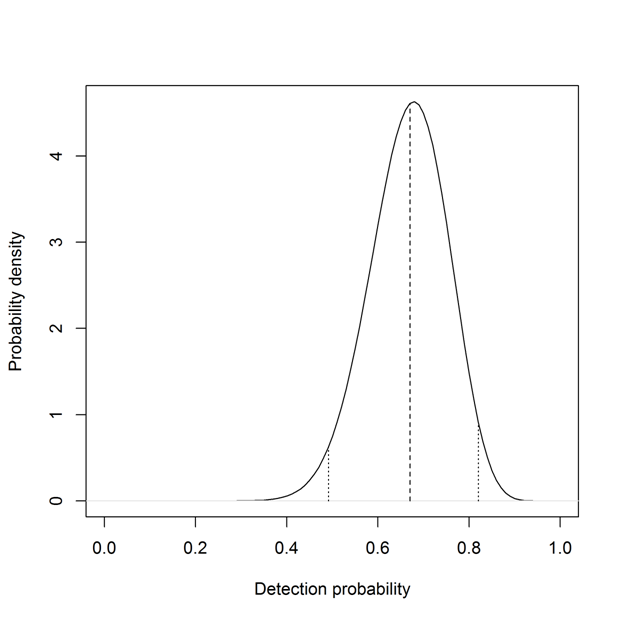
\includegraphics[height=2.5in]{Ch6/figs/densityvsdetection}
\end{center}
\caption{Probability density plot of a hypothetical posterior distribution of beta(20,10); dashed lines indicate mean and upper and lower 95\% interval}
\label{densityvsdetection.fig}
\end{figure}

The posterior distribution summarizes all we know about a parameter
and thus, is the central object of interest in Bayesian
analysis. Unfortunately, in many if not most practical applications,
it is nearly impossible to directly compute the posterior. Recall
Bayes’ theorem:
\begin{equation}
p(theta|y) = p(y|\theta) * p(\theta) / p(y),
\label{mcmc.eq.bayes}
\end{equation}
where $\theta$ is the parameter of interest, $y$ is the observed data,
$p(\theta|y)$ is the posterior, $p(y|\theta)$ the likelihood of the
data conditional on $\theta$, $p(\theta)$ the prior probability of
$\theta$, and, finally, $p(y)$ is the marginal probability of the
data, which can also be written as
\[
p(y) = \int p(y|\theta) * p(\theta) dtheta
\]

This marginal probability is a normalizing constant that ensures that
the posterior integrates to 1. You read in Chapter 2 that this
integral is often hard or impossible to evaluate, unless you are
dealing with a really simple model.  For example, consider that you
have a Normal model, with a set of n observations, $y$ that come from a
Normal distribution:
\[
 y \sim \mbox{Normal}(\mu, \sigma),
\]
where $\sigma$ is known and our objective is to obtain an estimate of
$\mu$ using Bayesian statistics. To fully specify the model in a Bayesian
framework, we first have to define a prior distribution for $\mu$. Recall
from Chapter 2 that for certain data models, certain priors lead to
conjugacy – i.e. if you choose the right prior for your parameter,
your posterior distribution will be of a known parametric form. The
conjugate prior for the mean of a normal model is also a Normal
distribution:
\[
\mu \sim \mbox{Normal}(\mu_0, \sigma_{0}^{2})
\]
If $\mu_{0}$ and $\sigma_{0}^{2}$ are fixed, the posterior for $\mu$ has the following form (for the algebraic proof, see XXX):
\begin{equation}
\mu|y \sim \mbox{Normal}(\mu_{n}, \sigma_{n}^{2})
\label{mcmc.eq.mu-posterior}
\end{equation}
where
\[
\mu_{n} =  (sig^2 / sig^2  +n* sig0^2)*  mu0 + (n * sig0^2 / sig^2  +n* sig0^2) *y-bar
\]
And
\[
 sign^2 = sig^2 * sig0^2 / (sig^2 + n*sig0^2)
\]
We can directly obtain estimates of interest from this Normal
posterior distribution, such as the mean mu-hat and its variance; we
do not need to apply MCMC, since we can recognize the posterior as a
parametric distribution, including the normalizing constant $p(y)$.
But generally we will be interested in more complex models with
several, say n, parameters. In this case, computing $p(y)$ from
Eq. \ref{mcmc.eq.bayes} requires n-dimensional integration, which is
can be difficult or impossible. Thus, the posterior distribution in
generally only known up to a constant of proportionality:
\[
p(\theta|y) propto p(y|\theta) * p(\theta)
\]
The power of MCMC is that it allows us to approximate the posterior
using simulation without evaluating the high dimensional integrals and
to directly sample from the posterior, even when the posterior
distribution is unknown! The price is that MCMC is computationally
expensive. Although MCMC first appeared in the scientific literature
in 1949 \citep{metropolis_etal:1949}, widespread use did not occur
until the 1980s when computational power and speed increased
\citep{gelfand_smith:1990}. It is safe to say that the advent of
practical MCMC methods is the primary reason why Bayesian inference
has become so popular during the past three decades.
In a nutshell, MCMC lets us generate sequential draws of $\theta$ (the
parameter(s) of interest) from distributions approximating the unknown
posterior over T iterations. The distribution of the draw at t depends
on the value drawn at t-1; hence, the draws from a Markov
chain. \footnote{In case you are not familiar with Markov chains, for
  t random samples $\theta$ (1), ... $\theta$ (t) from a Markov chain
  the distribution of $\theta$ (t) depends only on the most recent
  value, $\theta$ (t-1).} As T goes to infinity, the Markov chain
converges to the desired distribution – in our case the posterior
distribution for $\theta$|y. Thus, once the Markov chain has reached
its stationary distribution, the generated samples can be used to
characterize the posterior distribution, $p(\theta|y)$, and point
estimates of $\theta$, its standard error and confidence bounds, can
be obtained directly from this approximation of the posterior. In
practice, although we know that a Markov chain will eventually
converge, we can only generate a limited number of samples – a process
that depending on the model can be quite time consuming. Assessing
whether our Markov chain has indeed converged is an important part of
MCMC sampling and we will speak about some common diagnostics in
Section XX.



\section{Types of MCMC sampling}

There are several MCMC algorithms, the most popular being Gibbs
sampling and Metropolis-Hastings sampling. We will be dealing with
these two classes in more detail and use them to construct the MCMC
algorithms for SCR models. Also, we will briefly review alternative
techniques that are applicable in some situations.


\subsection{Gibbs sampling}

Gibbs sampling was named after the physicist J.W. Gibbs by
\citet{geman_geman:1984}, who applied the algorithm to a Gibbs
distribution \footnote{a distribution from physics we are not going to
  worry about, since it has no immediate connection with Gibbs
  sampling other than giving its name}. The roots of Gibbs sampling
can be traced back to work of \citet{metropolis_ulam:1953}, and it is
actually closely related to Metropolis sampling (see Chapter 11.5 in
\citet{gelman_etal:2004}, for the link between the two samplers). We
will focus on the technical aspects of this algorithm, but if you find
yourself hungry for more background, \citet{casella_george:1992}
provide a more in-depth introduction to the Gibbs sampler.

In Chapter 2 you already heard about the basic principles of Gibbs
sampling\footnote{maybe we should think out chapter 2 and concentrate
  that material here?}. But as a refresher, let's go back to our
simple example from above to understand the motivation and functioning
of Gibbs sampling. Recall that for a Normal model with known variance
and a Normal prior for $\mu$, the posterior distribution of $\mu|y$ is also
Normal. Conversely, with a fixed (known) $\mu$, but unknown variance, the
conjugate prior for $\sigma^2$ is an Inverse-Gamma distribution with shape and scale parameters $a$ and $b$:
\[
\sigma^2 \sim Iv-Gamma(a,b),
\]
With fixed $a$ and $b$, the posterior $p(sig|mu,y)$ is also an Inverse Gamma distribution, namely:
\begin{equation}
sig|\mu,y \sim Inv Gamma (an, bn),
\label{eq. 3}
\end{equation}
 where  $an = n/2   + a$ and $bn = 1/2 \sigma (yi-mu)^2+ b$
However, what if we know neither $mu$ nor $sig$, which is probably the
more common case? The joint posterior distribution of $mu$ and $sig$
now has the general structure
\[
p(mu, sig|y) = \frac{p(y|mu)* p(mu) *p(sig)}{ \int p(y|mu)* p(mu) *p(sig) dmu dsig }
\]
Or
\[
p(mu, sig|y) \propto p(y|mu)* p(mu) *p(sig)
\]
This cannot easily be reduced to a distribution we recognize. However,
we can condition mu on sig (i.e., we treat sig as fixed) and remove
all terms from the joint posterior distribution that do not involve mu
to construct the full conditional distribution,
\[
p(mu|sig,y)  \propto p(y|mu)* p(mu)
\]


The full conditional of mu again takes the form of the Normal
distribution shown in Eq. \ref{eq. 2}; similarly, $p(sig|mu,y)$ takes
the form of the Inverse Gamma distribution shown in
Eq. Eq. \ref{eq. 3}  – both distribution we can easily sample
from. And this is precisely what we do when using Gibbs sampling – we
break down high-dimensional problems into convenient one-dimensional
problems by constructing the full conditional distributions for each
model parameter separately; and we sample from these full
conditionals, which, if we choose conjugate priors, are known
parametric distributions.
Let's put the concept of Gibbs sampling into the MCMC framework of
generating successive samples, using our simple Normal model with
unknown mu and sig and conjugate priors as an example. These are the
steps you need to build a Gibbs sampler:

{\flushleft {\bf Step 0:} Begin with some initial values for $\theta$, $\theta$(0).   }
In our example, we have to specify initial values for mu and sig, for
example by drawing a random number from some uniform distribution, or
by setting them close to what we think they might be. (Note: This step
is required in any MCMC sampling – chains have to start from
somewhere. We will get back to these technical details a little
later.)
{\flushleft {\bf Step 1:} Draw $\theta$1(1) from the conditional distribution p($\theta$1(1)|$\theta$2(0),…, $\theta$d(0)) }
Here, $\theta$1 is mu, which we draw from the Normal distribution in Eq. \ref{eq. 2}  using sig(0) as value for sig.
{\flushleft Step 2: Draw $\theta$2(1) from the conditional distribution p($\theta$2(1)|$\theta$1(1), $\theta$3(0),…, $\theta$d(0)) }
Here, $\theta$2 is sig, which we draw from the Inverse Gamma
distribution of Eq. \ref{eq. 3}, using mu(1) as value for mu...

{\flushleft {\bf Step d:} Draw $\theta$d(1) from the conditional distribution p($\theta$d(1)|$\theta$1(1),..., $\theta$d-1(1)) }

In our example we have no additional parameters, so we only need step 0 through to 2.
Repeat Steps 1 to d for K = a large number of samples.
In terms of R coding, this means we have to write Gibbs updaters for
mu and sig and embed them into a loop over K iterations. The final
code in the form of an R function is shown in Panel 1.

\begin{verbatim}
Andy will build the panel environment here soon.

Panel 1: R-code for a Gibbs sampler for a Normal model with unknown mu
and sig and conjugate (Normal and Inverse Gamma, respectively) priors
for both parameters.

Normal.Gibbs<-function(y=y,mu0=mu0, sig0=sig0, a=a,b=b,niter=niter) {

ybar<-mean(y)
n<-length(y)
mu<-runif(1) #mean initial value
sig<-runif(1) #sd initial value
an<-n/2 + a

out<-matrix(nrow=niter, ncol=2)
colnames(out)<-c('mu', 'sig')

for (i in 1:niter) {

#update mu
mun<- (sig/(sig+n*sig0))*mu0 + (n*sig0/(sig+n* sig0))*ybar
sign <- (sig*sig0)/ (sig+n*sig0)
mu<-rnorm(1,mun, sqrt(sign))

#update sig
bn<- 0.5 * (sum((y-mu)^2)) +b
sig<-1/rgamma(1,shape=an, rate=bn)
out[i,]<-c(mu,sqrt(sig))

}
return(out)
}
\end{verbatim}

This is it! You can use the code \mbox{\tt NormalGibbs.R} in the {\bf
  R} package \mbox{\tt scrbook}
to simulate some data, $y \sim \mbox{Normal}(5, 0.5)$ and run your first
Gibbs sampler. Your output will be a table with two columns, one per
parameter, and $K$ rows, one per iteration. For this 2-parameter example
you can visualize the joint posterior by plotting samples of $\mu$
against samples of $\sigma$ (Fig. 2 XXX):
\begin{verbatim}
plot(out[,1], out[,2])
\end{verbatim}
The marginal distribution of each parameter is approximated by just
examining the samples of this particular parameter – you can visualize
it by plotting a histogram of the samples (Fig. 3 a, b XXX):
\begin{verbatim}
par(mfrow=c(1,2))
hist(out[,1]); hist (out[,2])
\end{verbatim}

Finally, recall an important characteristic of Markov chains, namely,
that the chain has to have converged (reached its stationary
distribution) for samples to come from the posterior distribution. In
practice, that means you have to throw out some of the initial samples
– called the burn-in. We will talk about this in more when we talk
about convergence diagnostics. For now, you can use the
\verb#plot(out[,1])# or \verb#plot(out[,2])# command to make a time
series plot of the samples of each parameter and visually assess how
many of the initial samples you should discard. Figure 3 c and d shows
plots for the estimates of mu and sigma from our simulated data set;
you see that in this simple example the Markov chain apparently
reaches its stationary distribution very quickly – the chains look
'grassy' seemingly from the start. It is hard to discern a burn-in
phase visually (but we will see examples further on where the burn-in
is clearer) and you may just discard the first 500 draws to be sure
you only use samples from the posterior distribution. The mean of the
remaining samples are your estimates of mu and sig:
\begin{verbatim}
> summary(mod[501:10000,])
       mu                      sig
 Min.   : 4.936      Min.   : 0.4569
 1st Qu.: 4.984     1st Qu.: 0.4889
 Median : 4.994   Median : 0.4961
 Mean   : 4.994    Mean   : 0.4964
 3rd Qu.: 5.005    3rd Qu.: 0.5037
 Max.   : 5.062      Max.   : 0.5356
\end{verbatim}

\begin{figure}
\begin{center}
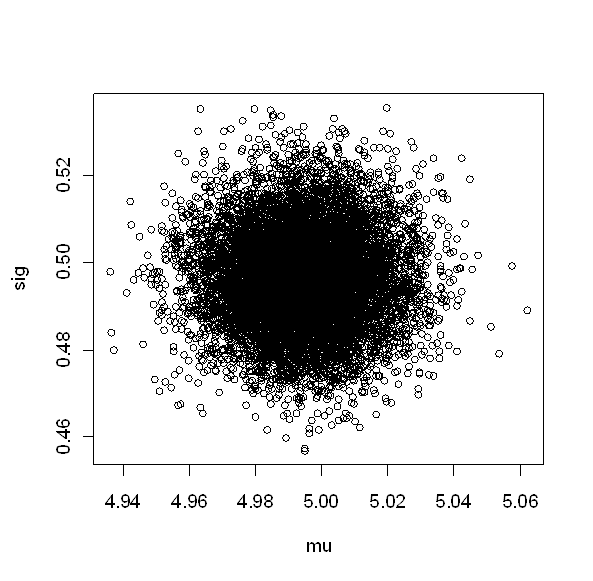
\includegraphics[height=3in]{Ch6/figs/postdist}
\end{center}
\caption{Joint posterior distribution of mu and sig from a Normal Model}
\label{postdist.fig}
\end{figure}

\begin{figure}
\begin{center}
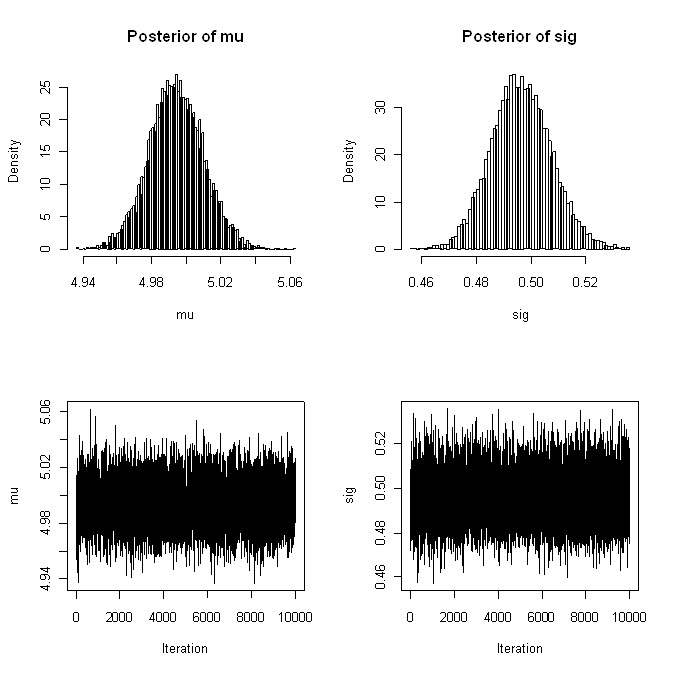
\includegraphics[width=2.5in]{Ch6/figs/plotsofPD}
\end{center}
\caption{Plots of the posterior distributions of mu(a) and sig (b)
  from a Normal model and time series plots of mu (c) and sig (d).}
\label{plotsofPD.fig}
\end{figure}

\subsection{ Metropolis-Hastings sampling   }

Although it is applicable to a wide range of problems, the limitations
of Gibbs sampling are immediately obvious – what if we do not want to
use conjugate priors (or what if we cannot recognize the full
conditional distribution as a parametric distribution, or simply do
not want to worry about these issues)? The most general solution is to
use the Metropolis-Hastings (MH) algorithm, which also goes back to
the work by \citet{metropolis_ulam:1953}. You saw the basics of this
algorithm in Chapter 2. In a nutshell, because we do not recognize the
posterior $p(\theta|y)$ as a parametric distribution, the MH algorithm
generates samples from a known proposal distribution, say $h(\theta)$,
that depends on $\theta$ at t-1. The $t^{th}$ sample is accepted or
rejected based on its joint posterior probability density compared to
the density of the sample at t-1. The original Metropolis algorithm
requires $h(\theta)$ to be symmetric so that
$h(\theta^{t}|\theta^{t-1}) = h(\theta^{t-1}|\theta^{t})$; but a later
development of the algorithm by \citet{hastings:1970} lifted this
condition. Using a symmetric proposal distribution makes life a little
easier and we are going to limit our coverage of the
Metropolis-Hastings sampler to this specific case. Specifically, we
are going to use a Normal proposal distribution, which is also
referred to as 'random walk Metropolis-Hastings sampling'. It is worth
knowing that there are alternative formulations of the algorithm. For
example, in the independent M-H, $\theta^{t}$ does not depend on
$\theta^{t-1}$, while the Langevin algorithm \citep{roberts_etal:1998}
aims at avoiding the random walk by favoring moves towards regions of
higher posterior probability density. The interested reader should
look up these algorithms in \citet{robert_casella:2004} or
\citet{robert_casella:2010}.

Building a MH sampler can be broken down into several steps. We are going to demonstrate these steps using a different but still simple and common model – the logit-normal or logistic regression model. For simplicity, assume that
\[
y \sim \mbox{Bern}(\exp(\theta)/(1+ exp(\theta)))
\]
and
\[
\theta \sim \mbox{Normal}(\mu_0, \sigma)
\]
The following steps are required to set up a random walk MH algorithm:

{\flushleft Step 0: Choose initial values, $\theta$(0).}

{\flushleft Step 1: Generate a proposed value of $\theta$ at t from h(thetat|thetat-1). }
We often use a Normal proposal distribution, so we draw $\theta$1 from $Normal(theta0, sigh^2)$, where $sigh^2$ is the variance of the Normal proposal distribution, a tuning parameter  that we have to set.

{\flushleft Step 2: Calculate the ratio of posterior densities for the proposed and the original value for $\theta$: }
\[
r = p(\theta^{t}|y) / p(\theta^{t-1}|y)
\]
In our example,
\[
r = \mbox{Bern}(y|\theta^{t}) * Normal(\theta^{t}|\mu_0, \sigma_0) / Bernoulli(y|thetat-1) * Normal(thetat-1|mu0, sig0)
\]
Step 3: Set
\begin{verbatim}
\begin{eqnarray*}
$\theta$ (t)  &= &   $\theta$ (t) \mbox{with probability min(r,1)}//
	 & = & 	$\theta$ (t-1) \mbox{ otherwise }
\end{eqnarray*}
\end{verbatim}
%this kept causing errors


We can do that by drawing a random number $u$ from a
$\mbox{Unif}(0,1)$ and accept $\theta^{t}$ if
$u<r$.
Repeat for $t = 1,2,\ldots$ a large number of samples.
The {\bf R} code for this MH sampler is provided in Panel 2 XXXX.
{\small
\begin{verbatim}
Panel 2: R code to run a Metropolis sampler on a simple Logit-Normal model.

Logreg.MH<-function(y=y, mu0=mu0, sig0=sig0, niter=niter) {

out<-c()

theta<-runif(1, -3,3) #initial value

for (iter in 1:niter){
theta.cand<-rnorm(1, theta, 0.2)

loglike<-sum(dbinom(y, 1, exp(theta)/(1+exp(theta)), log=TRUE))
logprior <- dnorm(theta,mu0 ,sig0, log=TRUE)
loglike.cand<-sum(dbinom(y, 1, exp(theta.cand)/(1+exp(theta.cand)), log=TRUE))
logprior.cand <- dnorm(theta.cand, mu0, sig0, log=TRUE)

if (runif(1)<exp((loglike.cand+logprior.cand)-(loglike+logprior))){
theta<-theta.cand
}
out[iter]<-theta
}

return(out)
}
\end{verbatim}
}

The reason we sum the logs of the likelihood and the prior, rather than multiplying the original values, is simply computational. The product of small probabilities can be numbers very close to 0, which computers do not handle well. Thus we add the logarithms, sum, and exponentiate to achieve the desired result. Similarly, in case you have forgotten some elementary math, $x/y = exp(log(x)-log(y))$, with the latter being favored for computational reasons.

Comparing MH sampling to Gibbs sampling, where all draws from the conditional distribution are used, in the MH algorithm we discard a portion of the candidate values, which inherently makes in less efficient than Gibbs sampling – the price you pay for its increased generality.
In Step 1 of the MH sampler we had to choose a variance for the Normal proposal distribution. Choice of the parameters that define our candidate distribution is also referred to as 'tuning', and it is important since adequate tuning will make your algorithm more efficient, i.e. your Markov chain will converge faster. The variance should be chosen so that (a) each step of drawing a new proposal value for $\theta$ can cover a reasonable distance in the parameter space, as otherwise, the random walk moves too slowly; and (b) proposal values are not rejected too often, as otherwise the random walk will 'get stuck' at specific values for too long.  As a rule of thumb, your candidate value should be accepted in about 40\% of all cases. Acceptance rates of 20 – 80\% are probably ok, but anything below or above may well render your algorithm inefficient (this does not mean that it will give you wrong results – only that you will need more iterations to converge to the posterior distribution). In practice, tuning will require some 'trial-and-error' and some common sense. Or, one can use an adaptive phase, where the tuning parameter is automatically adjusted until it reaches a user-defined acceptance rate, at which point the adaptive phase ends and the actual Markov chain begins. This is computationally a little more advanced. \citet{link_barker:2009} discuss this in more detail. It is important the samples drawn during the adaptive phase are discarded.
You can easily check acceptance rates for the parameters you monitor (that are part of your output) using the rejectionRate() function of the package coda (we will talk more about this package a little later on). Do not let the term 'rejection rate' confuse you; it is simply 1 – acceptance rate. There may be parameters – for example, individual values of a random effect or latent variables – that you do not want to save, though, and in our next example we will show you a way to monitor their acceptance rates with a few extra lines of code.

\subsection{ Metropolis-within-Gibbs }

One weakness of the MH sampler is that formulating the joint posterior when evaluating whether to accept or reject the candidate values for $\theta$ becomes increasingly complex or inefficient as the number of parameters in a model increases. It is probably going to sound like MCMC sampling is too good to be true – but in these cases you can simply combine MH sampling and Gibbs sampling. You can use Gibbs sampling to break down your high-dimensional parameter space into easy-to-handle one-dimensional conditional distributions and use MH sampling for these conditional distributions. Better yet – if you have some conjugacy in your model, you can use the more efficient Gibbs sampling for these parameters and one-dimensional MH for all the others. You have already seen the basics of how to build both types of algorithms, so we can jump straight into an example here and build a Metropolis-within-Gibbs algorithm.

\section{ GLMMs – Poisson regression with a random effect }

Let's assume a model that gets us closer to the problem we ultimately want to deal with – a GLMM. Here, we assume we have Poisson counts, y, from i plots in j different study sites, and we believe that the counts are influenced by some plot-specific covariate, x, but that there is also a random site effect. So our model is:
\[
yij \sim Poisson (lamij)
\]
\[
lamij = exp (aj + b*xi)
\]
Let's use Normal priors on a and b,  \[
aj \sim Normal (mua, siga)
\]
and
\[
b \sim Normal (mub, sigb)
\].
\footnote{Why is b a hyperparameter?}
Since we want to estimate the random effect in this model, we do not
specify $\mu_a$ and $\sigma_a$, but instead, estimate them as well, so we have
to specify hyperpriors for these parameters:
\begin{eqnarray*}
\mu_a  &\sim &  Normal(mu0, sig0)  \\
\sigma_{a} & \sim & InvGamma(a0, b0)
\end{eqnarray*}

With the model fully specified, we can compile the full conditionals, breaking the multi-dimensional parameter space into one-dimensional components:
\begin{verbatim}
\begin{eqnarray*}
p(a1|a2,a3,…aj,b,y)  & \propto  & p(yi1|a1,b) * p(a1|mua, siga) \\
	 & \propto &  Poisson(yi1| exp(a1 + b*x[j=1])) * Normal(a1|mua, siga)
\end{eqnarray*}
\begin{eqnarray*}
p(a2|a1,a3,…aj,b,y) & \propto&  p(yi2|a2,b) * p(a2|mua, siga) \\
	 & \propto  & Poisson(yi2|exp(a2 + b*x[j=1])) * Normal(a2|mua, siga)
\end{eqnarray}
and so on for all elements of a.
\begin{eqnarray*}
p(b|a,y) &\propto & p(y|a,b) * p(b) \\
	 &\propto& Poisson(y|exp(a + b*x)) *Normal(b|mub, sigb)
\end{eqnarray*}
\end{verbatim}
%couldn't get this to work either

Finally, we need to update the hyperparameters for a:
\[
p(mua|a) \propto p(a|mua, siga) *p(mua)
\]
\[
p(siga|a) \propto p(a|mua, siga) *p(siga)
\]
Since we assumed a to come from a Normal distribution, the choice of priors for mua – Normal – and siga – Inverse Gamma – leads to the same conjucagy we observed in our initial Normal model, so that both hyperparameters can be updated using Gibbs sampling.

Now let' build the updating steps for these full conditionals. Again, for the MH steps that update a and b we use Normal proposal distributions with standard deviations sigha and sighb.

First, we set the initial values a(0) and b(0). Then, starting with a1, we draw a1(1) from Normal (a1(0), sigha), calculate the conditional posterior density of a1(0) and a1(1) and compare their ratios,
\[
r = Poisson(y(j=1)|exp(a1(1) + b*x)) * Normal(a1(1)|mua, siga) / Poisson(y(j=1)|exp(a1(0) + b*x)) * Normal(a1(0)|mua, siga)
\]
and accept a1(1) with probability min(r,1). We repeat this for all a's.

For b, we draw b(1) from Normal (b(0), sigbh), compare the posterior densities of b(0) and b(1),
\[
r = Poisson(y|exp(a + b(1)*x)) *Normal(b(1)|mub,sigb) / Poisson(y|exp(a + b(0)*x)) *Normal(b(0)|mub,sigb),
\]
and accept b (1) with probability min(r,1).

For mua and siga, we sample directly from the full conditional distributions (Eq XX and Eq XX):
\[
mua(1) \sim Normal (mun, sign)
\]
where $mun =  (siga(0) / siga(0)  +na* sig0)*  mu0 + (na * sig0/ siga(0)  +na* sig0) *abar(1)
and sign= siga(0) * sig0/ (siga(0) + n*sig0)$
Here, abar is the current mean of the vector a, which we updated before, and na is the length of a. For siga we use $siga(1)\sim Inv Gamma (an, bn)$,
where  $an = na/2   + a0$, and $bn = 1/2 \Sigma (a(1)-mua(1))^2+ b0$.

We repeat these steps over K iterations of the MCMC algorithm.
In this example we may not want to save each value for a, but are only interested in their mean and standard deviation. Since these two parameters will change as soon as the value for one element in a changes, their acceptance rates will always be close to 1 and are not representative of how well your algorithm performs. To monitor the acceptance rates of parameters you do not want to save, you simply need to add a few lines of code into your updater to see how often the individual parameters are accepted. The full code for the MCMC algorithm of our Poisson GLMM in Panel 3 shows one way how to monitor acceptance of individual a's.

{\small
\begin{verbatim}
Panel 3: R code for the Metropolis-within-Gibbs sampler for
a Poisson regression with random intercepts.

Pois.reg<-function(y=y,site=site,mu0=mu0,sig0=sig0,a0=a0,b0=b0,
          mub=mub, sigb=sigb, niter=niter){

lev<-length(unique(site))     #number of sites
a<-runif(lev,-5,5)		#initial values a
b<-runif(1,0,5)			#initial value b
mua<-mean(a)
siga<-sd(a)

out<-matrix(nrow=niter, ncol=3)
colnames(out)<-c('mua','siga','b')

for (iter in 1:niter) {

#update a
aUps<-0			  #initiate counter for acceptance rate of a
for (j in 1:lev) { 	  #loop over sites
a.cand<-rnorm(1, a[j], 0.1)	#update intercepts a one at a time
loglike<- sum(dpois (y[site==j], exp(a[j] + b*x[site==j]), log=TRUE))
logprior<- dnorm(a[j], mua,siga, log=TRUE)
loglike.cand<- sum(dpois (y[site==j], exp(a.cand + b *x[site==j]), log=TRUE))
logprior.cand<- dnorm(a.cand,  mua,siga, log=TRUE)
if (runif(1)< exp((loglike.cand+logprior.cand) –(loglike+logprior))) {
a[j]<-a.cand
aUps<-aUps+1
}
}

if(iter %% 100 == 0) {  #this lets you check the acceptance rate of a at every 100th iteration
            cat("   Acceptance rates\n")
            cat("     a =", aUps/lev, "\n")
}

#update b
b.cand<-rnorm(1, b, 0.1)
avec<-rep(a, times=c(rep(10,10)))
loglike<- sum(dpois (y, exp(avec + b*x), log=TRUE))
logprior<- dnorm(b, mub,sigb, log=TRUE)
loglike.cand<- sum(dpois (y, exp(avec + b.cand *x), log=TRUE))
logprior.cand<- dunif(b.cand, mub,sigb, log=TRUE)
if (runif(1)< exp((loglike.cand+logprior.cand) – (loglike+logprior) )) {
b<-b.cand
}

#update mua using Gibbs sampling
abar<-mean(a)
mun<- (siga/(siga+lev*sig0))*mu0 + (lev*sig0/(siga+lev* sig0))*abar
sign <- (siga*sig0)/ (siga+lev*sig0)
mua<-rnorm(1,mun, sqrt(sign))

#update siga using Gibbs sampling
a0n<-lev/2 + a0
b0n<- 0.5 * (sum((a-mua)^2)) +b0
siga<-1/rgamma(1,shape=a0n, rate=b0n)

out[iter,]<-c(mua, sqrt(siga), b)

}

return(out)
}
\end{verbatim}
}

\subsection{Rejection sampling and slice sampling }

While MH and Gibbs sampling are probably the most widely applied algorithms for posterior approximation, there are other options that work under certain circumstances and may be more efficient when applicable. WinBUGS applies these algorithms and we want you to be aware that there is more out there to approximate posterior distributions than Gibbs and MH.
One alternative algorithm is rejection sampling. Rejection sampling is not an MCMC method, since each draw is independent of the others. The method can be used when the posterior $p(\theta|y)$ is not a known parametric distribution but can be expressed in closed form. Then, we can use a so-called envelope function, say, $g(\theta)$, that we can easily sample from, with the restriction that $p(\theta|y) < M * g(\theta)$. We then sample a candidate value for $\theta$ from $g(\theta)$, calculate $r = p(\theta|y)/M*g(\theta)$ and keep the sample with the probability r. M is a constant that has to be picked so that r E [0,1], for example by evaluating both $p(\theta|y)$ and $g(\theta)$ at n points and looking at their ratios. Rejection sampling only works well if $g(\theta)$ is similar to $p(\theta|y)$, and packages like WinBUGS use adaptive rejection sampling \citep{gilks_wild:1992}, where a complex algorithm is used to fit an adequate and efficient g(theta)based on the first few draws. Though efficient in some situations, rejection sampling does not work well with high-dimensional problems, since it becomes increasingly hard to define a reasonable envelope function. For an example of rejection sampling in the context of SCR models, see Chapter 9.
Another alternative is slice sampling \citep{neal:2003}. In slice sampling, we sample uniformly from the area under the plot of $p(\theta|y)$. Considering a single univariate theta. Let's define an auxiliary variable, $U \sim  Uniform(0, p(\theta|y))$. Then, $\theta$ can be sampled from the vertical slice of $p(\theta|y)$ at U (Figure 4):

\begin{verbatim}
\theta|U \sim \mbox{Unif}(B),
\end{verbatim}
where $B = {\theta: U < p(\theta|y)}$


\begin{figure}
\begin{center}
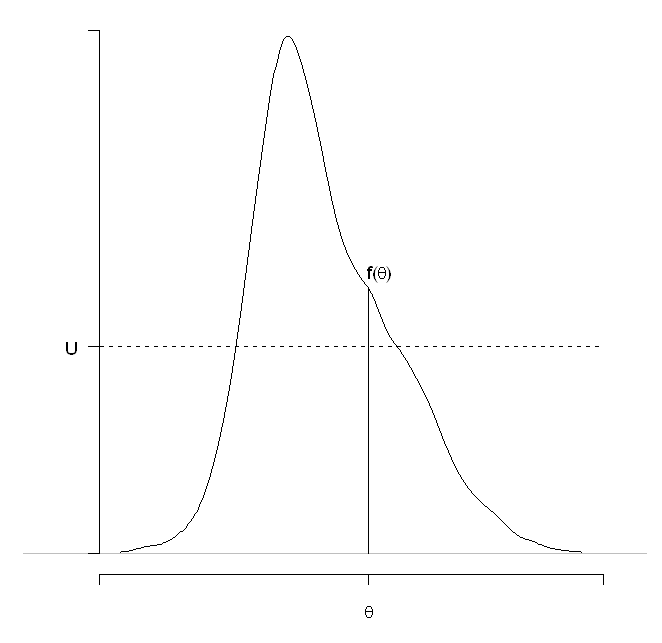
\includegraphics[height=2in]{Ch6/figs/slicesampling}
\end{center}
\caption{Slice sampling. For...}
\label{slicesample.fig}
\end{figure}

\footnote{there are supposed to be equations in the caption of figure
4 but it kept causing errors}

Slice sampling can be applied in many situations; however, implementing an efficient slice sampling procedure can be complicated. We refer the interested reader to chapter 7 of \citet{Robert_casella:2010} for a simple example.
Both rejection sampling and slice sampling can be applied on one-dimensional conditional distributions within a Gibbs sampling setup.
\section{MCMC for closed capture-recapture Model Mh}
\footnote{Andy could move material from chapter 3 to here.}


\section{MCMC algorithm for the basic spatial capture-recapture model}

By now you have seen how to build MCMC algorithms for some basic generalized linear models. Now, we'll walk you through the steps of building your own MCMC sampler for the basic SCR model (i.e. without any individual, site or time specific covariates) with both a Poisson and a binomial encounter process.
As usual, we will have to go through two general steps before we write the MCMC algorithm:

(1)Identify your model with all its components (including
    priors)

(2) Recognize and express the full conditiona ldistributions for
    all parameters

It is worthwhile to go through all of step 1 for an SCR model, but you
have probably seen enough of step 2 in our previous examples to get
the essence of how to express a full conditional
distribution. Therefore, we will exemplify step 2 for some parameters
and tie these examples directly to the respective R code.


{\bf Step 1 – Identify your model}

Recall the components of the basic SCR model with a Poisson encounter process from Chapter 3:
We assume that individuals i, or rather, their activity centers si, are uniformly distributed across our state space S,
\[
si  \sim U(S)
\]
and that the number of times individual i encounters trap j, yij, is a random Poisson variable with mean lamij,
\[
yij \sim Poisson(lamij)
\]
The tie between individual location, movement and trap encounter rates is made by the assumption that lamij, is a decreasing function of the distance between si and j, Dij, of the half-normal form
\[
Lamij =  lam0 * exp(-Dij2/2*sig2),
\]
where lam0 is the baseline trap encounter rate at $Dij=0$ and sig controls the shape of the half-normal function.

In order to estimate the number of si in S, N, we use data augmentation (sect. 3.XYZ) and create M-n all-0 encounter histories, where n is the number of individuals we observed and M is an arbitrary number that is larger than N. We estimate N by summing over the auxiliary data augmentation variables, zi, which is 1 if the individual is part of the population and 0 if not, and assume that zi is a random Bernoulli variable,
\[
z_{i} \sim \mbox{Bern}(\psi)
\]


To link the two model components, we modify our trap encounter model to
\[
Lamij = lam0 * exp(-Dij2/2*sig2) * zi.
\]
The model has the following structural parameters, for which we need to specify priors
$\psi$ – the Uniform (0,1) is required as part of the data augmentation procedure and in general is a natural choice of an uninformative prior for a probability; note that this is equivalent to a Beta(1,1) prior, which will come in handy later.
$s_{i}$ – since si is a pair of coordinates it is two-dimensional and we use a uniform prior limited by the extent of our state-space over both dimensions.
$\sigma$ – we can conceive several priors for sigma but let's assume an improper prior – one that is Uniform over (-Inf, Inf). We will see why this is convenient when we construct the full conditionals for sigma.
$\lambda_{0}$ – analogous, we will use a Uniform (-Inf, Inf) improper prior for sigma.
The parameter that is the objective of our modeling, N, is a derived parameter that we can simply obtain by summing all z's:
\[
N=sum(z)
\]


{\bf Step 2 - Construct the full conditionals}
Having completed step 1, let's look at the full conditional distributions for some of these parameters.
We find that with improper priors, full conditionals are proportional only to the likelihood of the observations; for example, take the movement parameter sigma:
\[
Sig|s, lam0, z, y propto [y| s, lam0, z, sig] * [sig]
\]
Since the improper prior implies that [sig] propto 1, we can reduce this further to
\[
Sig|s, lam0, z, y propto [y| s, lam0, z, sig]
\]
The R code to update sigma is shown in Panel 4. \footnote{ Somewhere in chapter 2 i added a comment about rejecting parameters outside of the parameter space as being an ok thing to do. Richard said he read something in Robert and Casella’s book on that. Hopefully he can remember where and we can cite it back in Ch 2 and again here.  It could be mentioned in a sentence or two up in the MCMC section.}

{\small
\begin{verbatim}
Panel 4: R code to update sigma within an MCMC algorithm for
an SCR model when using an improper prior


sig.cand <- rnorm(1, sigma, 0.1)	#draw candidate value
 if(sig.cand>0){   #automatically reject sig.cand that are <0
     lam.cand <- lam0*exp(-(D*D)/(2*sig.cand*sig.cand))
     ll<- sum(dpois(y, lam*z, log=TRUE))
     llcand <- sum(dpois(y, lam.cand*z, log=TRUE))
     if(runif(1) < exp( llcand  - ll) ){
         ll<-llcand
         lam<-lam.cand
         sigma<-sig.cand
      }
  }

\end{verbatim}
}
These steps are analogous for lam0 and si and we will use MH steps for
all of these parameters. Similar to the random intercepts in our
Poisson GLMM, we update each si individually. Note that to be fully
correct, the full conditional for si contains both the likelihood and
prior component, since we did not specify an improper, but a Uniform
prior on si. However, with a Uniform distribution the probability
density of any value is 1/(upper limit – lower limit) =
constant. Thus, the prior components are identical for both the
current and the candidate value and can be ignored (formally, when you
calculate the ratio of posterior densities, r, the identical prior
component appears both in the numerator and denominator, so that they
cancel each other out).

We still have to update zi. The full conditional for zi is
\[
zi|y, sigma, lam0, s propto [y|z,sigma, lam0, s] * [zi]
\]
and since $zi \sim Bernoulli(psi)$,
the term has to be taken into account when updating zi. The R code for updating zi is shown in Panel 5.

{\small
\begin{verbatim}
Panel 5: R code to update z…

        zUps <- 0		#set counter to monitor acceptance rate
        for(i in 1:M) {
            if(seen[i])	#no need to update seen individuals, since their z =1
                next
            zcand <- ifelse(z[i]==0, 1, 0)
            llz <- sum(dpois(y[i,],lam[i,]*z[i], log=TRUE))
            llcand <- sum(dpois(y[i,], lam[i,]*zcand, log=TRUE))

            prior <- dbinom(z[i], 1, psi, log=TRUE)
            prior.cand <- dbinom(zcand, 1, psi, log=TRUE)
            if(runif(1) < exp( (llcand+prior.cand) - (llz+prior) )) {
                z[i] <- zcand
                zUps <- zUps+1
            }
        }
\end{verbatim}
}

$\psi$
itself is a hyperparameter of the model, with an uninformative prior distribution of Unif(0,1) or Beta(1,1), so that
\[
Psi|z \propto [z|psi] * Beta(1,1)
\]
The Beta distribution is the conjugate prior to the Binomial and Bernoulli distributions (remember that $z \sim Bernoulli(psi))$. The general form of a full conditional of a Beta-Binomial model with $yi \sim Bernoulli (p) $ and $p \sim Beta(a,b) $ is
\[
p(p|y) \propto Beta(a + sum(yi), b + n-sum(yi)))
\]
In our case, this means we update psi as follows:
\begin{verbatim}
si<-rbeta(1, 1+sum(z), 1 + M-sum(z))
\end{verbatim}

These are all the building blocks you need to write the MCMC algorithm
for the spatial null model with a Poisson encounter process.  You can
find the full R code (SCR0pois.R) in the online supplementary
material.

\subsection{SCR model with binomial encounter process}
The equivalent SCR model with a binomial encounter process is very similar. Here, each individual i can only be detected once at any given trap j during a sampling occasion k.
Thus
\[
yij \sim Binomial (pij, K)
\]
Where $p_{ij}$ is some function of distance between ${\bf s}_{i}$ and trap location ${\bf x}_{j}$. Here we use:
\[
pij=1-exp(-lamij)
\]
Recall from Chapter 2 that this is the complementary log-log (cloglog) link function, which constrains pij to fall between 0 and 1.
For our MCMC algorithm that means that, instead of using a Poisson likelihood, $Poisson(y|sigma,lam0,s,z)$, we use a Binomial likelihood, $Binomial(y,K|sigma,lam0,s,z)$, in all the conditional distributions. As an example, Panel 6 shows the updating step for lam0 under a binomial encounter model. The full MCMC code for the binomial SCR can be found in the online supplements.

{\small
\begin{verbatim}
Panel 6: MCMC updater for lam0 in a SCR model with Binomial encounter
process and cloglog link function on detection. Here, pmat =
1-exp(-lam).

        lam0.cand <- rnorm(1, lam0, 0.1)
        if(lam0.cand >0){   #automatically reject lam0.cand that are <0
            lam.cand <- lam0.cand*exp(-(D*D)/(2*sigma*sigma))
            p.cand <- 1-exp(-lam.cand)
            ll<- sum(dbinom(y, K, pmat *z, log=TRUE))
            llcand <- sum(dbinom(y, K, p.cand *z, log=TRUE))
            if(runif(1) < exp( llcand  - ll) ){
                ll<-llcand
                pmat<-p.cand
                lam0<- lam0.cand
            }
        }
\end{verbatim}
}

Another possibility is to model variation in the individual and site specific detection probability, pij, directly, without any transformation, such that
\begin{verbatim}
pij<-p0 * exp(-Dij2/(2*sig^2))
\end{verbatim}
and $p0 = \{0,1\}$.
This formulation is analogous to how detection probability is modeled in distance sampling under a half-normal detection function; however, in distance sampling p0 - detection of an individual on the transect line - is assumed to be 1 \citep{buckland_etal:2001}. Under this formulation the updater for lam0 (equivalent to p0 in Eq XX) becomes:
\begin{verbatim}
        lam0.cand <- rnorm(1, lam0, 0.1)
        if(lam0.cand >0 & lam0.cand < 1 ){   #automatically reject lam0.cand that are not {0,1}
            lam.cand <- lam0.cand*exp(-(D*D)/(2*sigma*sigma))
            ll<- sum(dbinom(y, K, lam *z, log=TRUE)) #no transformation needed
            llcand <- sum(dbinom(y, K, lam.cand *z, log=TRUE))
            if(runif(1) < exp( llcand  - ll) ){
                ll<-llcand
                lam<-lam.cand
                lam0<- lam0.cand
            }
        }
\end{verbatim}


\subsection{Looking at model output}
Now that you have an MCMC algorithm to analyze spatial capture-recapture data with, let's run an actual analysis so we can look at the output. As an example, we will use the bear data ... \footnote{Does this data set come up before Ch6? If not, introduce data here. Or, Andy, would you rather use simulated data?} You can use the same script provided back in Chapter XX to read in the data and build the augmented encounter history array; then source the MCMC code for the binomial encounter model algorithm with the cloglog link and run 5000 iterations. This should take approximately 25 minutes.
\begin{verbatim}
> source('SCR0binom.txt')
> mod0<-SCR.0(y=bigTrap, X=trapmat, M=M, xl=xl, xu=xu, yl=yl, yu=yu, K=8, niter=5000)
\end{verbatim}

Before, we used simple R commands to look at model results. However, there is a specific R package to summarize MCMC simulation output and perform some convergence diagnostics – package coda \citep{plummer_etal:2006}. Download and install coda, then convert your model output to an mcmc object
\begin{verbatim}
> chain<-mcmc(mod0)
\end{verbatim} which can be used by coda to produce MCMC specific output.

\subsubsection{Markov chain time series plots}
Start by looking at time series plots of your Markov chains using \verb#plot(chain)#. This command produces a time series plot and marginal posterior density plots for each monitored parameter, similar to what we did before using the \verb#hist()# and \verb#plot()# commands (Fig. 5). Time series plots will tell you several things:
First, the way the chains move through the parameter space gives you an idea of whether your MH steps are well tuned. If chains were constant over many iterations you would probably need to decrease the tuning parameter of the (Normal) proposal distribution. If a chain moves along some gradient to a stationary state very slowly, you may want to increase the tuning parameter so that the parameter space is explored more efficiently.


\begin{figure}
\begin{center}
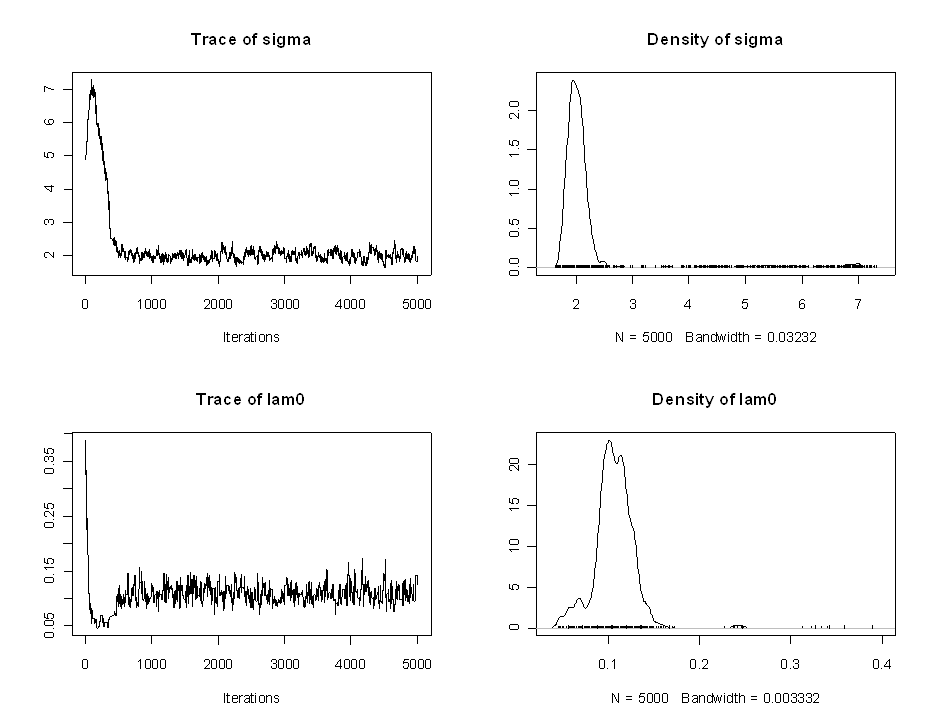
\includegraphics[height=2.5in]{Ch6/figs/timeseries}
\end{center}
\caption{Time series and posterior density plots for sigma and lam0.}
\label{timeseries.fig}
\end{figure}


Second, you will be able to see if your chains converged and how many initial simulations you have to discard as burn-in. In the case of the chains shown in Figure 5, we would probably consider the first 750 - 1000 iterations as burn-in, as afterwards the chains seem to be fairly stationary.

\subsubsection{A word of caution about chain convergence }
Since we do not know what the stationary posterior distribution of our Markov chain should look like (this is the whole point of doing an MCMC approximation), we effectively have no means to assess whether it has converged to this desired distribution or not. As mentioned before, the only certainty is that a Markov chain will {\it eventually} converge to its stationary distribution, but no-one can tell us how long this will take. Also, you only now the part of your posterior distribution that the Markov chain has explored so far– for all you know the chain could be stuck in a local maximum, while other maxima remain completely undiscovered.  Acknowledging that there is truly nothing we can do to ever proof convergence of our MCMC chains, there are several things we can do to increase the degree of confidence we have about the convergence of our chains. One option, and that advocated by what we will loosely call the WinBUGS community, is to run several Markov chains and to start them off at different initial values that are overdispersed relative to the posterior distribution. Such initial values help to explore different areas of the parameter space simultaneously; if after a while all chains oscillate around the same average value, chances are good that they indeed converged to the posterior distribution. Gelman and Rubin came up with a diagnostic statistic that essentially compares within-chain and between-chain variance to check for convergence of multiple chains \citep{gelman_etal:2004}. Of course, running several parallel chains is computationally expensive.
Extra computational demands are not the only and by no means the major concern some people voice when it comes to running several parallel MCMC chains to assess convergence. Again, consider the fact that we do not know anything about the true form of the posterior distribution we are trying to approximate. How do we, then, know how to pick overdispersed initial values? We don’t – all we can do is pick overdispersed values relative to our expectations of what the posterior should look like. To use a quote from the home page of Charlie Geyer, a Bayesian statistician from the University of Minnesota, ``If you don't know any good starting points [...], then restarting the sampler at many bad starting points is [...] part of the problem, not part of the solution.'' (http://users.stat.umn.edu/~charlie/mcmc/diag.html). His suggestion is that your only chance to discover a potential problem with your MCMC sampler is to run it for a very long time. But again, there is no way of knowing how long is long enough.
It is up to you to decide, which school of thoughts appeals more to you – one long versus several parallel Markov chains. Irrespectively, part of developing an MCMC sampler should be to make sure (within reasonable limits) that you are not missing regions of high posterior density because of the way you specify your starting values. Once you have explored the behavior of your chain under a – reasonable – range of starting values, you may feel comfortable enough to run only one long chain.
The fact that convergence cannot be proven does not mean that you should not look for potential problems in your MCMC sampler. Some problems are easily detected using simple plots, such as the time series plots we discussed above. If the overall trajectory of your chain at the end of your simulations is still upward or downward, your chain clearly has not converged and you need to run your model much longer.  If you run several parallel chains and their stationary distributions look different, you may be looking at a multi-modal posterior – or a problem with your sampler. With these words of caution, let's get back to looking at our model output.

\subsection{Posterior density plots}
The plot() command also produces posterior density plots and it is worthwhile to look at those carefully. For parameters with priors that have bounds (e.g. Uniform over some interval), you will be able to see if your choice of the prior is truncating the posterior distribution. In the context of SCR models, this will mostly involve our choice of M, the size of the augmented data set. If the posterior of N has a lot of mass concentrated close to M (or equivalently the posterior of psi has a lot of mass concentrated close to 1), as in the example in Figure 6, we have to re-run the analysis with a larger M.  A flat posterior plot shows you that the parameter essentially cannot be identified – there may not be enough information in your data to estimate model parameters and you may have to consider a simpler model. Finally, posterior density plots will show you if the posterior distribution is symmetrical or skewed – if the distribution has a heavy tail, using the mean as a point estimate of your parameter of interest may be biased and you may want to opt for the median or mode instead.

\begin{figure}
\begin{center}
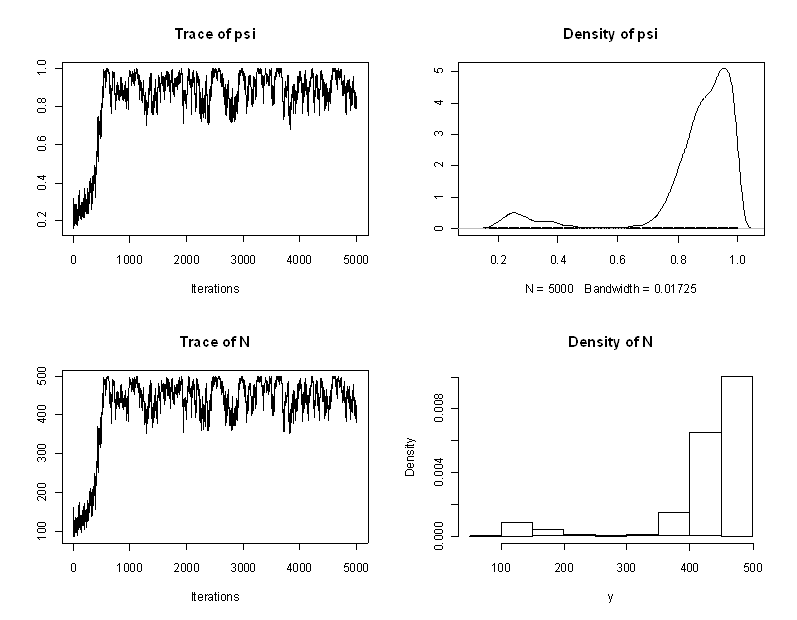
\includegraphics[height=2.5in]{Ch6/figs/timeseries2}
\end{center}
\caption{Time series and posterior density plots of psi and N for th
  ebear data set truncated by the upper limit of M (500).}
\label{timeseries2.fig}
\end{figure}

\subsection{Serial autocorrelation and effective sample size}
Even when we can be relatively confident that our chains have converged, the subsequent samples generated from a Markov chain are not iid samples from the posterior distribution, due to the correlation amongst samples introduced by the Markov process. As a consequence, the variance of the mean cannot simply be derived with the standard variance estimator, which takes into account the sample size (here, number of iterations). Rather, the sample size has to be adjusted to account for the autocorrelation in subsequent samples (see Chapter 8 in \citet{Robert_casella:2010} for more details). This adjusted sample size is referred to as the effective sample size. Checking the degree of autocorrelation in your Markov chains and estimating the effective sample size your chain has generated should be part of evaluating your model output. If you use WinBUGS through the R2WinBUGS package, the print() command will automatically return the effective sample size for all monitored parameters. In the coda package there are several functions you can use to do so. effectiveSize() will directly give you an estimate of the effective sample size for you parameters:
\begin{verbatim}
> effectiveSize(chain)
    sigma      lam0       psi         N
 3.930303 78.259159 30.436348 32.047392
\end{verbatim}

Alternatively, you can use the autocorr.diag() function, which will show you the degree of autocorrelation for different lag values (which you can specify within the function call, we use the defaults below):
\begin{verbatim}
> autocorr.diag(mcmc(mod))
           sigma      lam0       psi         N
Lag 0  1.0000000 1.0000000 1.0000000 1.0000000
Lag 1  0.9979948 0.9494134 0.9847503 0.9774201
Lag 5  0.9915567 0.8038168 0.9111951 0.9113525
Lag 10 0.9836016 0.6714021 0.8462108 0.8509803
Lag 50 0.8985337 0.1983780 0.6138516 0.6233994
\end{verbatim}
Whichever function you use, if you find that your supposedly long Markov chain has not generated enough pseudo-iid samples, you should consider a longer run. In the present case we see that autocorrelation is especially high for the parameter sigma and our effective sample size for this parameter is 4! \footnote{Anyone have any idea how the autocorrelation in sigma could be reduced?} This means we would have to run the model for much longer to obtain a reasonable effective sample size. Unfortunately, with many SCR models we observe high degrees of serial autocorrelation, which means we have to run long chains to obtain enough samples that can be considered iid, in order to obtain reasonable estimates of our parameters and their variances.
What exactly constitutes a reasonable effective sample size is hard to say, but as a rule of thumb you should probably aim at several hundreds of these pseudo-iid samples. A more meaningful measure of whether you've run your chain for enough iterations is the time-series or Monte Carlo error – the 'noise' introduced into your samples by the stochastic MCMC process – which we introduced in Chapter 2. The MC error decreases with increasing sample size and its magnitude can thus be controlled by adjusting the length of the Markov chain. As a rule of thumb, the MC error should be 1\% or less of the parameter estimate. Once you have reached this level, the estimates of the mean, standard error and 95\% quantiles should no longer change significantly with additional iterations. For highly correlated samples, it will take more iterations to reduce the MC error. In coda, the MC error is given as part of the summary results (see below).
 Another option to deal with the serial autocorrelation of samples is to 'thin' Markov chains by some rate r and save only every r-th iteration. But as discussed in Chapter 2, this is not efficient and should only be applied if needed for practical reasons (e.g. a large number of parameters and iterations may force you to thin your samples so you object storing the model output does not become unmanageably large).
For now, let's continue using this small set of samples to continue looking at the output.

\subsection{Summary results}
Now that we checked that our chains apparently have converged and pretending that we have generated enough samples from the posterior distribution, we can look at the actual parameter estimates. The summary() function will return two sets of results: the mean parameter estimates, with their standard deviation, the naïve standard error - i.e. your regular standard error calculated for K (= number of iterations) samples without accounting for serial autocorrelation - and the corrected MC error (Time-series SE), which accounts for autocorrelation. In WinBUGS, this latter value is referred to as MC error and is only given in the log output within BUGS itself.
You should adjust the summary() call by removing the burn-in from
calculating parameter summary statistics. To do so, use the window()
command, which lets you specify at which iteration to start
'counting'. In contrast to WinBUGS, which requires you to set the
burn-in length before you run the model, this command gives us full
flexibility to make decisions about the burn-in after we have seen the
trajectories of our Markov chains. For our example,
summary(window(chain, start=1001)) returns the following output:


\begin{verbatim}
Iterations = 1001:5000
Thinning interval = 1
Number of chains = 1
Sample size per chain = 4000

1. Empirical mean and standard deviation for each variable,
   plus standard error of the mean:

          Mean       SD  Naive SE Time-series SE
sigma   1.9986  0.13805 0.0021827       0.016091
lam0    0.1096  0.01523 0.0002407       0.001401
psi     0.6113  0.09148 0.0014465       0.010734
N     489.8535 71.79695 1.1352094       8.431119

2. Quantiles for each variable:

           2.5%       25%      50%      75%    97.5%
sigma   1.75780   1.89847   1.9900   2.0944   2.2772
lam0    0.08357   0.09824   0.1087   0.1192   0.1427
psi     0.45110   0.54838   0.6052   0.6639   0.8192
N     366.00000 440.00000 485.0000 530.0000 654.0000
\end{verbatim}

Looking at the MC errors, we see that in spite of the high autocorrelation, the MC error for sigma is below the 1%-threshold, whereas for all other parameters, MC errors are still above – another indication that for a thorough analysis we should run a longer chain.
Our algorithm gives us a posterior distribution of N, but we are usually interested in the density, D. Density itself is not a parameter of our model, but we can derive a posterior distribution for D by dividing each value of N (N at each iteration) by the area of the state-space (here 3032.719 km2) and we can use summary statistics of this distribution to characterize D:
\begin{verbatim}
> summary(window(chain[,4]/ 3032.719, start=1001))
Iterations = 1001:5000
Thinning interval = 1
Number of chains = 1
Sample size per chain = 4000

1. Empirical mean and standard deviation for each variable,
   plus standard error of the mean:

          Mean             SD       Naive SE Time-series SE
     0.1615229      0.0236741      0.0003743      0.0027801

2. Quantiles for each variable:

  2.5%    25%    50%    75%  97.5%
0.1207 0.1451 0.1599 0.1748 0.2156
\end{verbatim}
If we compare our mean density of $0.16/km2$ (and other parameters) with results from the same model run in secr and WinBUGS in Chapter XX, we see that estimates are almost identical (Table 1).


\subsection{Other useful commands }
While inspecting the time series plot gives you a first idea of how well you tuned your MH algorithm, use rejectionRate() to obtain the rejection rates (1 – acceptance rates) of the parameters that are written to your output:
\begin{verbatim}
> rejectionRate(chain)
     sigma       lam0        psi          N
0.44108822 0.77675535 0.00000000 0.01940388
\end{verbatim}
 Recall that rejection rates should lie between 0.2 and 0.8, so our tuning seems to have been appropriate here. Psi is never rejected since we update it with Gibbs sampling, where all candidate values are kept. And since N is the sum of all z, all it takes for N to change from one iteration to the next are small changes in the z-vector, so the rejection rate of N is always low.
If you have run several parallel chains, you can combine them into a single mcmc object using the mcmc.list() command on the individual chains (note that each chain has to be converted to an mcmc object before combining them with mcmc.list()). You can then easily obtain the Gelman-Rubin diagnostic \citep{gelman_etal:2004}, in WinBUGS called R-hat, using gelman.diag(), which will indicate if all chains have converged to the same stationary distribution.
For details on these and other functions, see the coda manual, which can be found –together with the package – on the CRAN mirror.

\section{Manipulating the state-space}
So far, we have constrained the location of the activity centers to fall within the outermost coordinates of our rectangular state space by posing upper and lower bounds for x and y. But what if S has an irregular shape – maybe there is a large water body we would like to remove from S, because we know our terrestrial study species does not occur there. Or the study takes place in a clearly defined area such as an island. As mentioned before, this situation is difficult to handle in WinBUGS. In some simple cases we can adjust the state space by setting SXi to be some function of SYi or vice versa. In this manner, we can cut off corners of the rectangle to approximate the actual state space. In R, we are much more flexible, as we can use the actual state-space polygon to constrain out si. \footnote{ Have to check if we can use panther stuff for the book; otherwise, use raccoon example.}To illustrate that, let's look at a camera trapping study of Florida panthers (Puma concolor coryi) conducted in the Picayune Strand Restoration Project (PSRP) area, southwest Florida (Fig. 7), by XXX, and financed by XXX. In the 1960ies the PSRP area was slated for housing development, but then bought back by the State of Florida and is currently being restored to its original hydrology and vegetation. In an effort to estimate the density of the local Florida panther population, 98 camera traps were operated in the area for 21 months between 2005 and 2007. Florida panthers are wide-ranging animals and in order to account for their wide movements, the state-space was defined as the trapping grid buffered by 15 km around its outermost coordinates. However, the resulting rectangle contained some ocean in its southwestern corner (Fig. 7).
In order to precisely describe the state-space, the ocean has to be removed. You can create a precise state-space polygon in ArcGIS and read it into R, or create the polygon directly within R. In the present case we intersected two shape files – one of the state of Florida and one of the rectangle defined by a strip of 15 km around the camera-trapping grid.
While you will most likely have to obtain the shapefile describing the landscape of and around your trapping grid (coastlines, water bodies etc.) from some external source, a polygon shapefile buffering your outermost trapping grid coordinates can easily be written in R.

If xmin, xmax, ymin and ymax, mark the outermost x and y coordinates of your trapping grid and b is the distance you want to buffer with, load the package shapefiles \citep{stabler:2006} and use:
\begin{verbatim}
xl= xmin-b
xu= xmax+b
yl= ymin-b
yu= ymax+b

dd <- data.frame(Id=c(1,1,1,1,1),X=c(xl,xu,xu,xl,xl),Y=c(yl,yl,yu,yu,yl)) #create data frame with coordinate pairs
ddTable <- data.frame(Id=c(1),Name=c("Item1"))
ddShapefile <- convert.to.shapefile(dd, ddTable, "Id", 5) #convert #to shapefile, type polygon
write.shapefile(ddShapefile, 'c:/…’, arcgis=T) # save to location of #choice
\end{verbatim}


\begin{figure}
\begin{center}
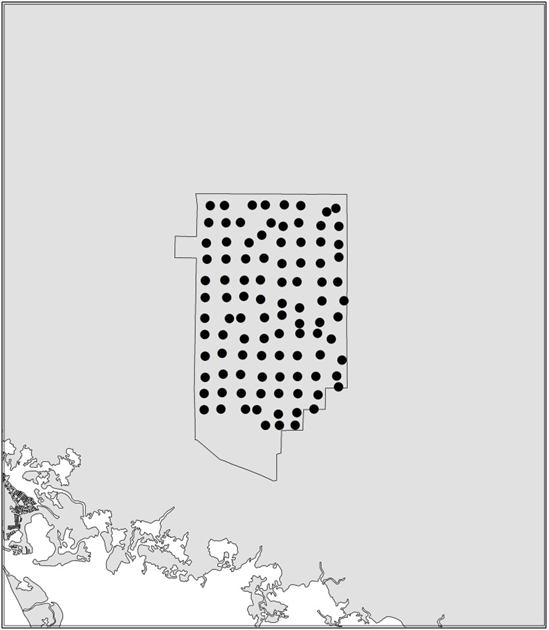
\includegraphics[height=2.5in]{Ch6/figs/panthercamera}
\end{center}
\caption{Rectangular state-space for a Florida panther camera trapping
study in the PSRP area (grey outline, red block inset map of Florida)
contain some ocean (white) that needs to be removed from the state-space.}
\label{pantercamera.fig}
\end{figure}

You can read shapefiles into R loading the package maptools
\citep{lewin-koh_etal:2011} and using the function
readShapeSpatial(). Make sure you read in shapefiles in UTM format, so
that units of the trap array, the movement parameter sigma and the
state-space are all identical.  Intersection of polygons can be done
in R also, using the package rgeos \citep{bivand_rundel:2011} and the
function gIntersect(). The area of your – single - polygon can be
extracted directly from the state-space object SSp:

\begin{verbatim}
> area <- SSp@polygons[[1]]@Polygons[[1]]@area /1000000
\end{verbatim}

 Note that dividing by 1000000 will return the area in km2 if your coordinates describing the polygon are in UTM. If your state-space consists of several disjunct polygons, you will have to sum the areas of all polygons to obtain the size of the state-space.
To include this polygon into our MCMC sampler we need one last spatial R package – sp \citep{pebesma_bivand:2011}, which has a function, over(), which allows us to check if a pair of coordinates falls within a polygon or not. All we have to do is embed this new check into the updating steps for s:
\begin{verbatim}
        Scand <- as.matrix(cbind(rnorm(M, S[,1], 2),
                   rnorm(M, S[,2], 2)))	        #draw candidate value

	Scoord<-SpatialPoints(Scand*1000)    #convert to spatial points on UTM (m) scale
	SinPoly<-over(Scoord,SSp)		# check if scand is within the polygon

       for(i in 1:M) {
	if(is.na(SinPoly[i])==FALSE) {		#if scand falls within polygon, continue update
… [rest of the updating step remains the same]
\end{verbatim}
Note that it is much more time-efficient to draw all M candidate values for s and check once if they fall within the state-space, rather than running the over() command for every individual pair of coordinates. To make sure that our initial values for s also fall within the polygon of S, we use the function runifpoint() from the package spatstat \citep{baddeley_turner:2005}, which generates random uniform points within a specified polygon. You'll find this modified MCMC algorithm in the online supplementary material (SCR0poisSSp).
Finally, observe that we are converting candidate coordinates of S back to meters to match the UTM polygon. In all previous examples, for both the trap locations and the activity centers we have used UTM coordinates divided by 1000 to estimate sigma on a km scale. This is adequate for wide ranging individuals like bears. In other cases you may center all coordinates on 0. No matter what kind of transformation you use on your coordinates , make sure to always convert candidate values for S back to the original scale (UTM) before running the over() command.

\section{MCMC software packages}
Throughout most of this book we will use WinBUGS and, occasionally, JAGS to run MCMC analyses. Here, we will briefly discuss the main pros and cons of these two programs as well as WinBUGS successor OpenBUGS. You can find scripts to simulate data and run the basic SCR model in all three programs in the online supplementary material (simSCR0poisBUGS).

\subsection{WinBUGS}
In a nutshell, WinBUGS (and the other programs) do everything that we just went through in this chapter (and quite a bit more). Looking through your model, WinBUGS determines which parameters it can use standard Gibbs sampling for (i.e. for conjugate full conditional distributions). Then, it determines, in the following hierarchy, whether to use adaptive rejection sampling, slice sampling or – in the 'worst' case – Metropolis-Hastings sampling for the other full conditionals \citep{spiegelhalter_etal:2003}. If it uses MH sampling, it will automatically tune the updater so that it works efficiently.
While WinBUGS is a convenient piece of software that is still widely used, its major drawback is that it is no longer being developed, i.e. no new functions or distributions are added and no bugs are fixed.

\subsection{OpenBUGS}
OpenBUGS is essentially the successor of WinBUGS. While the latter is
no longer worked on, OpenBUGS is constantly developed further. The
name 'OpenBUGS' refers to the software being open source, so users do
not need to download a license key, like they have to for WinBUGS
(although the license key for WinBUGS is free and valid for life).

Compared to WinBUGS, OpenBUGS has a lot more built-in functions. The
method of how to determine the right updater for each model parameter
has changed and the user can manually control the MCMC algorithm used
to update model parameters.  Several other changes have been
implemented in OpenBUGS and a detailed list of differences between the
two BUGS versions, can be found at
http://www.openbugs.info/w/OpenVsWin

While OpenBUGS is a useful program for a lot of MCMC sampling
applications, for reasons we do not understand, simple SCR models do
not converge in OpenBUGS. It is therefore advisable that you check any
OpenBUGS SCR model results against result from WinBUGS. Also,
currently, the R package BRugs \citep{thomas_etal:2006} – necessary
for running OpenBUGS through R – has problems with 64-bit machines, so
you may have to use the 32-bit version of R and OpenBUGS in order to
make it work. The BUGS project site at http://www.openbugs.info
provides a lot of information on and download links for OpenBUGS.

There is an extensive help archive for both WinBUGS and OpenBUGS and you can subscribe to a mailing list, where people pose and answer questions of how to use these programs at http://www.mrc-bsu.cam.ac.uk/bugs/overview/list.shtml

\subsection{JAGS – Just Another Gibbs Sampler}
JAGS, currently at Version 3.1.0, is another free program for analysis of Bayesian hierarchical models using MCMC simulation. Originally, JAGS was the only program using the BUGS language that would run on operating systems other than the 32 bit Windows platforms. By now, there are OpenBUGS versions for Linux or Macintosh machines.
JAGS 'only' generates samples from the posterior distribution; analysis of the output is done in R – either by running JAGS through R using either the packages rjags \citep{plummer:2011} or R2jags \citep{su_yajima:2011}, or by using coda on your JAGS output. The program, manuals and rjags can be downloaded at http://sourceforge.net/projects/mcmc-jags/files/
When run from within R using the package rjags or R2jags, writing a JAGS model is virtually identical to writing a WinBUGS model. However, some functions may have slightly different names and you can look up available functions and their use in the JAGS manual. One potential downside is that JAGS can be very particular when it comes to initial values. These may have to be set as close to truth as possible for the model to start. Although JAGS lets you run several parallel Markov chains, this characteristic interferes with the idea of using overdispersed initial values for the different chains. Also, we have occasionally experienced JAGS to crash and take the R GUI with it. Only re-installing both JAGS and rjags seemed to solve this problem.
On the plus side, JAGS usually runs a little faster than WinBUGS, sometimes considerably faster (see section 4.XYZ), is constantly being developed and improved and it has a variety of functions that are not available in WinBUGS. For example, JAGS allows you to supply observed data for some deterministic functions of unobserved variables. In BUGS we cannot supply data to logical nodes. Another useful feature is that the adaptive phase of the model (the burn-in) is run separately from the sampling from the stationary Markov chains. This allows you to easily add more iterations to the adaptive phase if necessary without the need to start from 0. There are other, more subtle differences and there is an entire manual section on differences between JAGS and OpenBUGS.
For questions and problems there is a JAGS forum online at http://sourceforge.net/projects/mcmc-jags/forums/forum/610037.
\footnote{As we make progress on the book, lets be sure  to add linkages to places where we use JAGS in examples.}

\section{Summary and Outlook}
While there are a number of flexible and extremely useful software packages to perform MCMC simulations, it sometimes is more efficient to develop your own MCMC algorithm. Building an MCMC code follows three basic steps: Identify your model including priors and express full conditional distributions for each model parameter. If full conditionals are parametric distributions, use Gibbs sampling to draw candidate parameter values from this distributions; otherwise use Metropolis-Hastings sampling to draw candidate values from a proposal distribution and accept or reject them based on their posterior probability densities.
These custom-made MCMC algorithms give you more modeling flexibility than existing software packages, especially when it comes to handling the state-space: In BUGS (and JAGS for that matter) we define a continuous rectangular state-space using the corner coordinates to constrain the Uniform priors on the activity centers s. But what if a continuous rectangle isn't an adequate description of the state-space? In this chapter we saw that in R it only takes a few lines of code to use any arbitrary polygon shapefile as the state-space, which is especially useful when you are dealing with coastlines or large bodies of water that need removing from the state-space. Another example is the SCR R package SPACECAP \citep{gopalaswamy_etal:2011} that was developed because implementation of an SCR model with a discrete state-space was inefficient in WinBUGS.
Another situations in which using BUGS/JAGS becomes increasingly complicated or inefficient is when using point processes other than the Uniform Poisson point process which underlies the basic SCR model (see Chapter X). In the Chapters 9 and XX you will see examples of different point processes, implemented using custom-made MCMC algorithms. \footnote{Richard, Beth expand on that?}
Finally, the Chapters XX and XX deal with unmarked or partially marked populations using hand-made MCMC algorithms to handle the (partially) latent individual encounter histories. While some of these models can be written in BUGS/JAGS, \footnote{the Poisson one for partially marked we wrote in BUGS and it should work with a known number of marked; the Bernoulli in JAGS with the dsum() function should work for the fully unknown; maybe some others? I don’t remember. We may have to try writing the others before saying that they don’t work in BUGS/JAGS; they are certainly much faster in R, though.}, they are painstakingly slow; others cannot be implemented in BUGS/JAGS at all.
In conclusion, while you can certainly get by using BUGS/JAGS for standard SCR models, knowing how to write your own MCMC sampler allows you to tailor these models to your specific needs.
